% Search for all the places that say "PUT SOMETHING HERE".

\documentclass[11pt]{article}
\usepackage{amsmath,textcomp,amssymb,geometry,graphicx,enumerate}

\def\Name{Sean Medin}  % Your name


\title{Modeling Evolution with Changing Selection Pressure}
\author{\Name}
\pagestyle{myheadings}
\date{}

\textheight=9in
\textwidth=6.5in
\topmargin=-.75in
\oddsidemargin=0.25in
\evensidemargin=0.25in

\graphicspath{{pics/}}


\begin{document}
\maketitle

\section*{Birth Rate Equation}

	\begin{equation*}
			(\frac{m_k}{n}(b_0 + r_0(m,n))e^{\frac{-1}{C_0}\sum{\frac{m_i}{n}}} + \frac{n - m_k}{n}(b_1 + r_1(m,n))e^{\frac{-1}{C_1}\sum{\frac{n - m_i}{n}}})e^{\frac{-N}{C_2}}
		\end{equation*}
		
\section*{Built in Features of System}

\begin{enumerate}

	\item
	The mutual resource ($C_2$) is small enough and/or the rewards ($a_i$) for homogeneity are large enough that when:
	
	\begin{equation} \label{eq:1}
		(b_i + a_i)e^{-N(\frac{1}{C_i} + \frac{1}{C_2})} \approx d
	\end{equation}
	
	where $i$ represents the dominant food source, we also have the condition that:
	
	\begin{equation*}
		b_je^{-\frac{N}{C_2}} < d
	\end{equation*}
	
	\item
	$b_0 + a_0 \approx b_1 + a_1$ so that consuming each of the foods are roughly equally beneficial for a single organism.
	
	\item
	The above feature is only true in the limit that $C_0,C_1,C_2 >> 1$ except when we are decreasing $C_0$.
	
\end{enumerate}
	
	

\section*{Stable Equilibrium}

Equilibrium is reached when the birth rate is equal to the death rate. For a system with a small mutation rate, a positive reward, and several genes, there are only two stable equilibrium positions.

	\begin{enumerate}
		
		\item
		The wide majority of the organisms (typically more than 90\%) consume a single food source. There are some organisms with one or two mutations away from that food source (due to the fact that the organisms always have some chance of mutating), but those dwindle quickly to 0 with the number of mutations leading away from consuming that food resource increase.
		
		\item
		Two genotypes dominate: one for each of the two food resources. Like in the last case, some in between genotypes are present, but in very low numbers.
		
	\end{enumerate}
	
	For the first case, we will be at an equilibrium when the birth rate of the organisms consuming all of one food is equal to the death rate.	We can find the approximate total population by solving for $N$ in equation \ref{eq:1}. For these simulations, $N \approx 11500$. We will also have a small number of organisms with a genotype one mutation away. The number of these can be found approximately using the following equation:
	
	\begin{equation*}
		\mu N d = a_iN_1e^{-N(\frac{1}{C_0} + \frac{1}{C_i})}
	\end{equation*}
	
	where $N_1$ is the population of organisms one mutation away from the dominant genotype. Plugging in the numbers predicts that we'd have $N_1 \approx 350$. The number of organisms with other genotypes is typically in the single digits. An example population graph over time is below:
	
	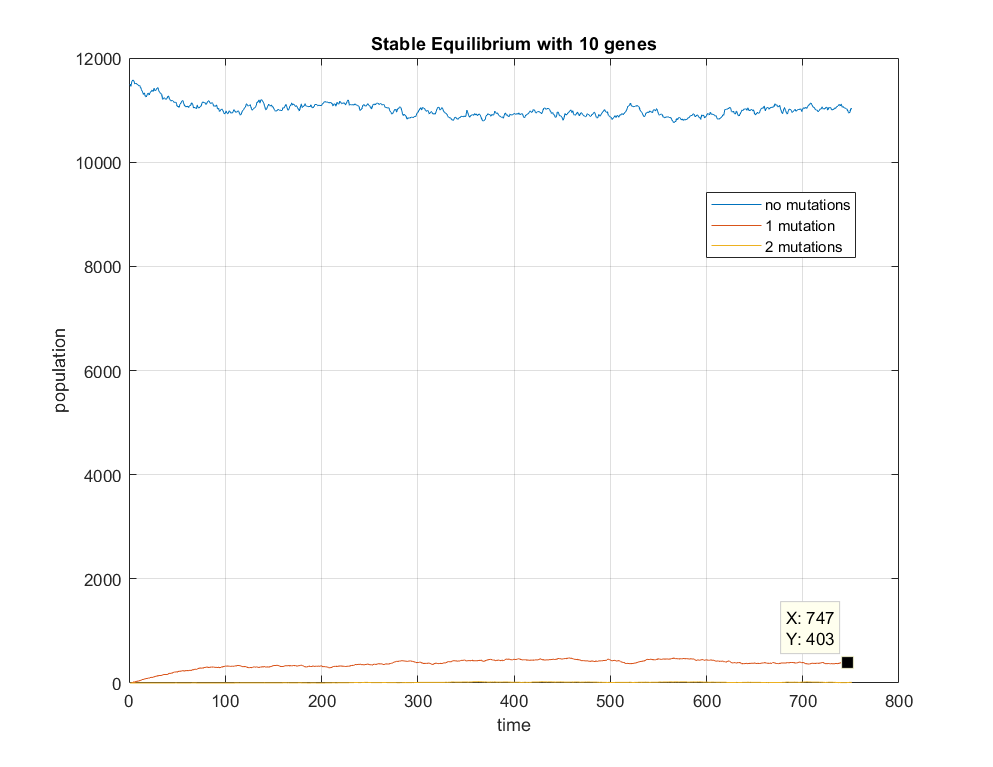
\includegraphics[scale = .8]{stable_equil}

\section*{Unstable Equilibrium}

	While there are technically many equilibria involving large numbers of organisms that don't have the two `pure' genotypes (in fact, one of them would have any of the two `pure' genotypes), none of them are stable. This is because neutral drift will always eventually lead to the one or both of the homogenous genotypes showing up and, due to the extra reward for being homogenous, they will inevitably out compete all the other genotypes. An example graph is below (10 genes, with the initial population being at an equilibrium with every organism having half of their genes being beneficial for one of the food resources): 
	
	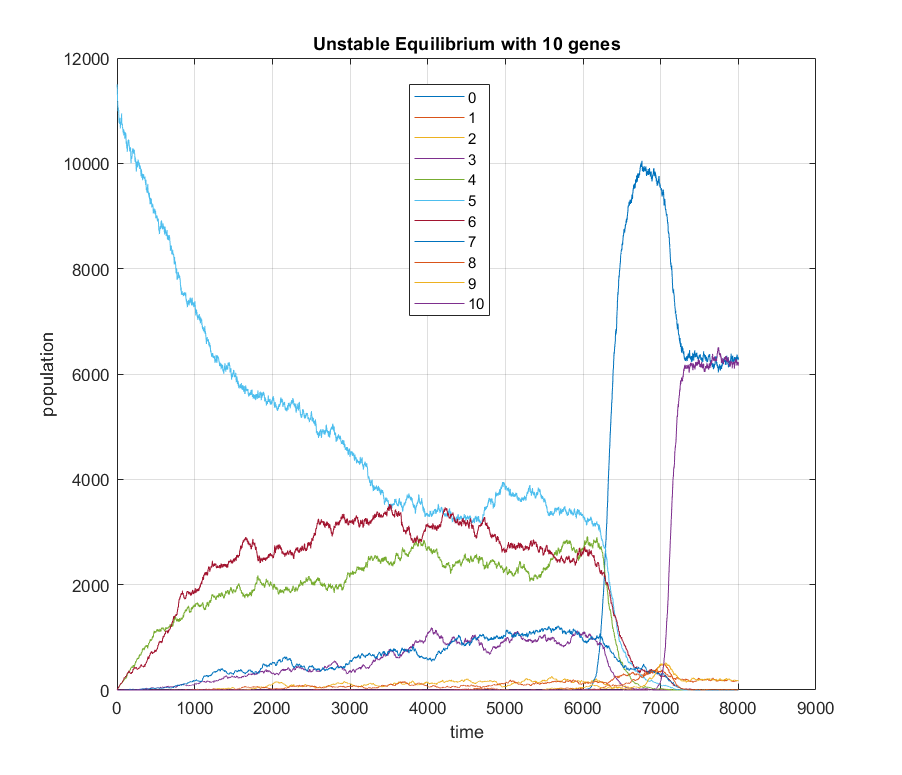
\includegraphics[scale = .8]{unstable_equil}

\section*{Sample Evolution}

	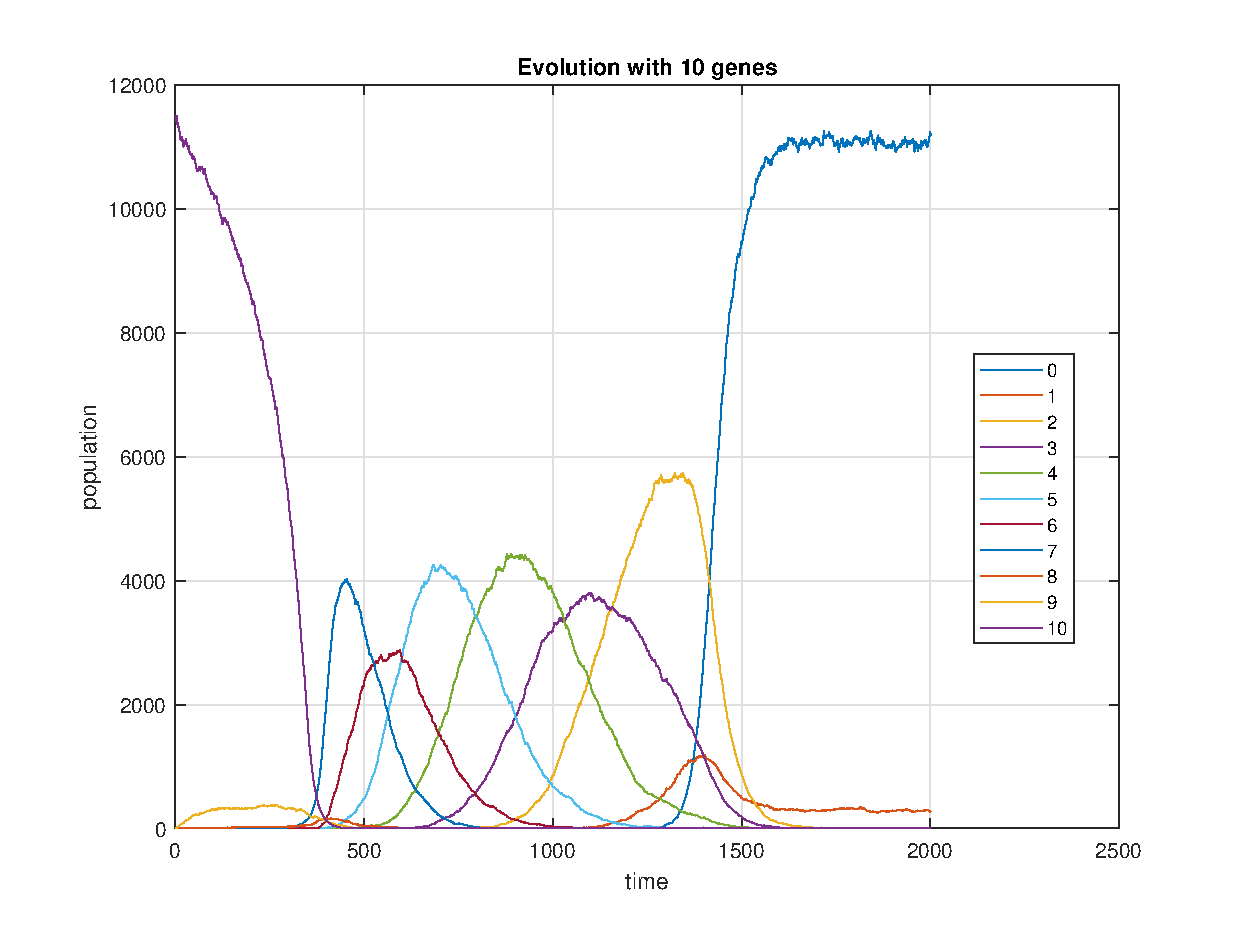
\includegraphics[scale = .8]{evolution_ex}

\section*{Time Until New Equilibrium Versus Number of Genes}

\section*{Original Food Decline and Return}

\subsection*{Case 1: Original Food Wins}

\subsection*{Case 2: New Food Wins}

\subsection*{Case 3: Coexistence}


\end{document}
